\item \points{2ci} {\bf Run ICL on XSum}

Now let's evaluate several different prompt formats on the XSum dataset. With and without a task description in the prompt, evaluate zero-shot and few-shot performance for XSum on GPT-2-Medium with the command:

\texttt{\small python3 main.py --task run\_icl --model med,full --dataset xsum --k 0,1,4 \textbackslash \\
\phantom{asdf}--prompt none,tldr,custom}

Note that we use much smaller $k$ than in the previous problem, because we must fit all $k$ examples into the model's context window, which is only 1024 tokens. The fixed context window length is one limitation of in-context learning.

\textbf{The $k=4$ XSum evaluation on full-size GPT-2 may take approximately 40 minutes on your Azure instance for each prompt mode}; this is expected, and is another downside of in-context learning (we need to process a much longer input, containing the prompt, compared to a fine-tuned model that just processes the test input).

Plot the zero-shot and few-shot performance of GPT-2 on XSum:

\texttt{\small python3 main.py --task plot\_icl --model med,full --dataset xsum --k 0,1,4 \textbackslash \\
\phantom{asdf}--prompt none,tldr,custom}

Your plot should look like:
\begin{figure}[H]
    \centering
    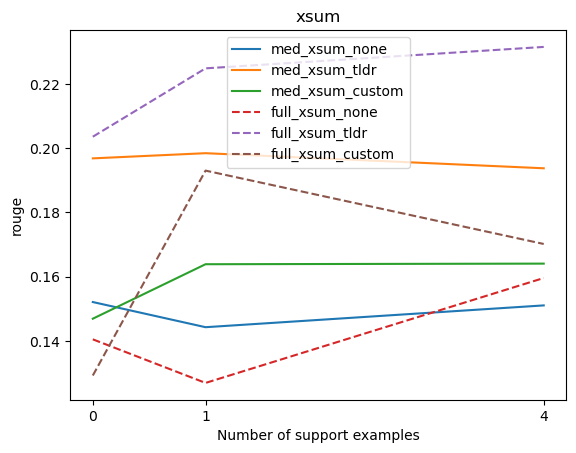
\includegraphics[width=0.75\linewidth]{./figures/q2_xsum_plot}
    \caption{\textit{k}-shot in-context performance of GPT-2-medium and full-size GPT-2 for various values of \textit{k} on XSum}
\end{figure}

